\documentclass{article}
\usepackage{tikz}
\def\bk{.5cm}
\newcommand\xeptang[2][0]{
	\foreach \i [evaluate=\i as \n using #2+1-\i]
	in {1,...,#2} {
		\foreach \j in {1,...,\n} {
			\draw[xshift=#1] ({(2*\j-2+\i)*\bk},{sqrt(3)*\i*\bk})node[]{$\bullet$} circle (\bk);
		};
	}
}
\begin{document}
	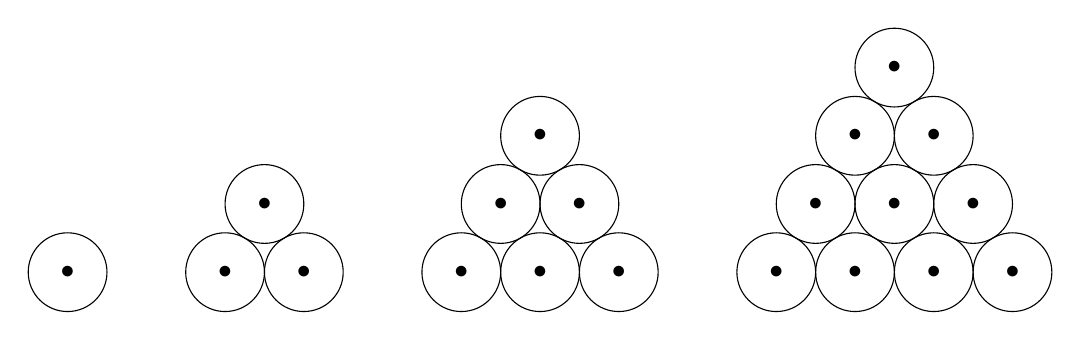
\begin{tikzpicture}
		\xeptang{1}
		\xeptang[2cm]{2}
		\xeptang[5cm]{3}
		\xeptang[9cm]{4}
	\end{tikzpicture}
\end{document}